\chapter{Introduction au domaine}
Ce TER, Android au pays des liseuses, fait appel à plusieurs technologies. Dans cette partie, nous allons nous intéresser a ces différentes technologies afin de préciser les avantages et les inconvénients de chacune d'entre elles.

\section{Les écrans E-ink}
L'E-Ink est une technologie d'écran qui permet de construire des écrans offrant de nombreux avantages.

\subsection{Avantages}
La consommation d'énergie très limitée. En effet, les écrans E-Ink ne consomment de l'énergie que pour mettre à jour l'affichage. Ainsi, ces écrans n'ont pas de rétro-éclairage ce qui apporte un confort visuel proche du papier en ne fatigue pas les yeux du lecteur. 

\subsection{Inconvéniants}
Par contre, les écrans E-Ink, ont une durée de rafraîchissement très longue ce qui est pénalisant pour afficher des animations par exemple. On estime que pour rafraîchir entièrement et "proprement" un écran de 7 pouces, il faut environ 1 seconde. Ce problème peut être limité en ne rafraîchissant qu'une petite partie de l'écran ou en effaçant pas entièrement l'affichage précédent. 

\subsection{Les écrans électrophorétiques}
Plusieurs technologies existent pour les écrans E-Ink, comme les écrans à cristaux liquides bistables, les écrans électrophorétiques ou encore les écrans polychromatiques. Nous allons nous intéresser plus particulièrement aux écrans électrophorétiques.\\

La liseuse à laquelle nous nous intéressons (Sony PRS-T1) possède un écran utilisant la technologie de l'électrophorétique.

L'écran possède des micro-capsules contenant des particules blanches chargées négativement ainsi que des particules noires chargées positivement. Lorsque l'on applique un champ électrique négatif, les particules blanches et noires se sépares (les blanches vont vers une extrémité de la capsule et les noires vers l'autre). Ainsi avec plusieurs millions de capsules et en appliquant des champs électriques, on peut afficher une image en noire et blanc. Une fois que la capsule à reçu un signal électrique, celle-ci garde son état.

Cette technologie à pour principal avantage sa très faible consommation d'énergie puisqu'une fois l'image chargée, elle reste telle qu'elle sans consommation d'énergie et ne nécessite pas d'éclairage particulier (la lumière ambiante suffit).

\begin{center}
	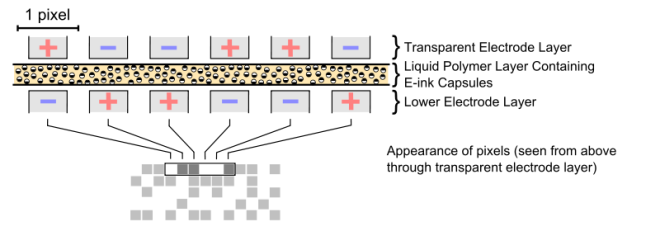
\includegraphics{Electrophoretic.png}
\end{center}


\section{Android}
Android est un système d'exploitation open source utilisant le noyau Linux, pour terminaux mobiles conçu par Android, une start-up rachetée par Google, et annoncé officiellement le 5 novembre 2007.

\subsection{Android pour liseuses}
Pour les liseuses, Android permet une adaptation relativement simple. L'avantage principal étant le système open-source qui permet de pouvoir modifier le middleware, comme montré dans l'exemple dans le cas de Freescale.\\
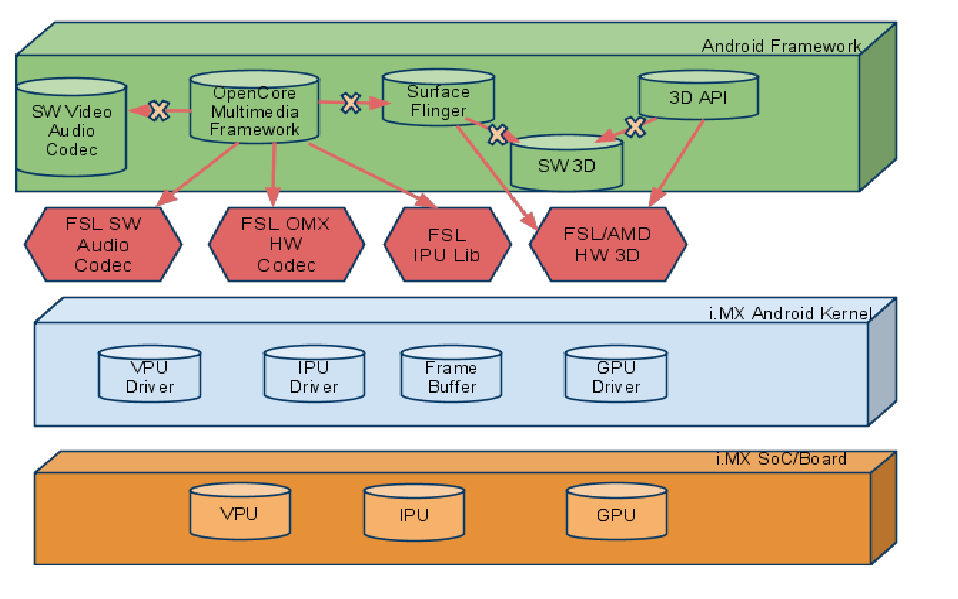
\includegraphics[scale=0.45]{Android.png}

\newpage

\section{Handheld devices}
Les handheld devices regroupe l'ensemble des terminaux mobiles. Ce qu'il faut noter en particulier avec ces terminaux c'est le mode de fonctionnement un peu différent des ordinateurs dit 'de bureau'. En effet, par économie d'espace et d'énergie, les constructeurs ont recours aux solutions System on Chip (SoC).

\subsection{System on Chip}
Un SoC est un système complet embarqué sur une puce, pouvant comprendre de la mémoire, un ou plusieurs microprocesseurs, des périphériques d'interface, ou tout autre composant nécessaire à la réalisation de la fonction attendue.
\\On retrouve ces systèmes embarquées dans divers produits comme des téléphones, des imprimantes, des systèmes de navigation pour voiture, des tablettes numériques et bien évidemment sur des liseuses.